\documentclass[a4paper,twoside,draft]{article}

\usepackage[utf8]{inputenc}
\usepackage[english,activeacute]{babel}
\usepackage{xspace}
\usepackage{graphicx}
\usepackage{verbatim}

\newcommand{\version}{0.1}
\newcommand{\ncurses}{\texttt{NCURSES}\xspace}
\newcommand{\DOM}{\texttt{DOM}\xspace}
\title{
  Robotic Turtles \version :\\
  Adapting a table-board game
  for computers \\
  {\tiny DRAFT VERSION}
}
\author{Rafael Mart\'inez Torres}
\begin{document}
\maketitle{}
\begin{abstract}
  Investing some extra time on analysis and design can make you save a
  lot of messy code, reaching even an astonishing \(O(1)\)
  development. This is the case when you use \ncurses library trying
  to adapt a table-board traditional game.
\end{abstract}

\section{Introduction}
\label{sec:intro}

Character Displays\cite{rockkind} are nowadays almost obsolete, due
\dots


\begin{comment}
  \begin{figure}
    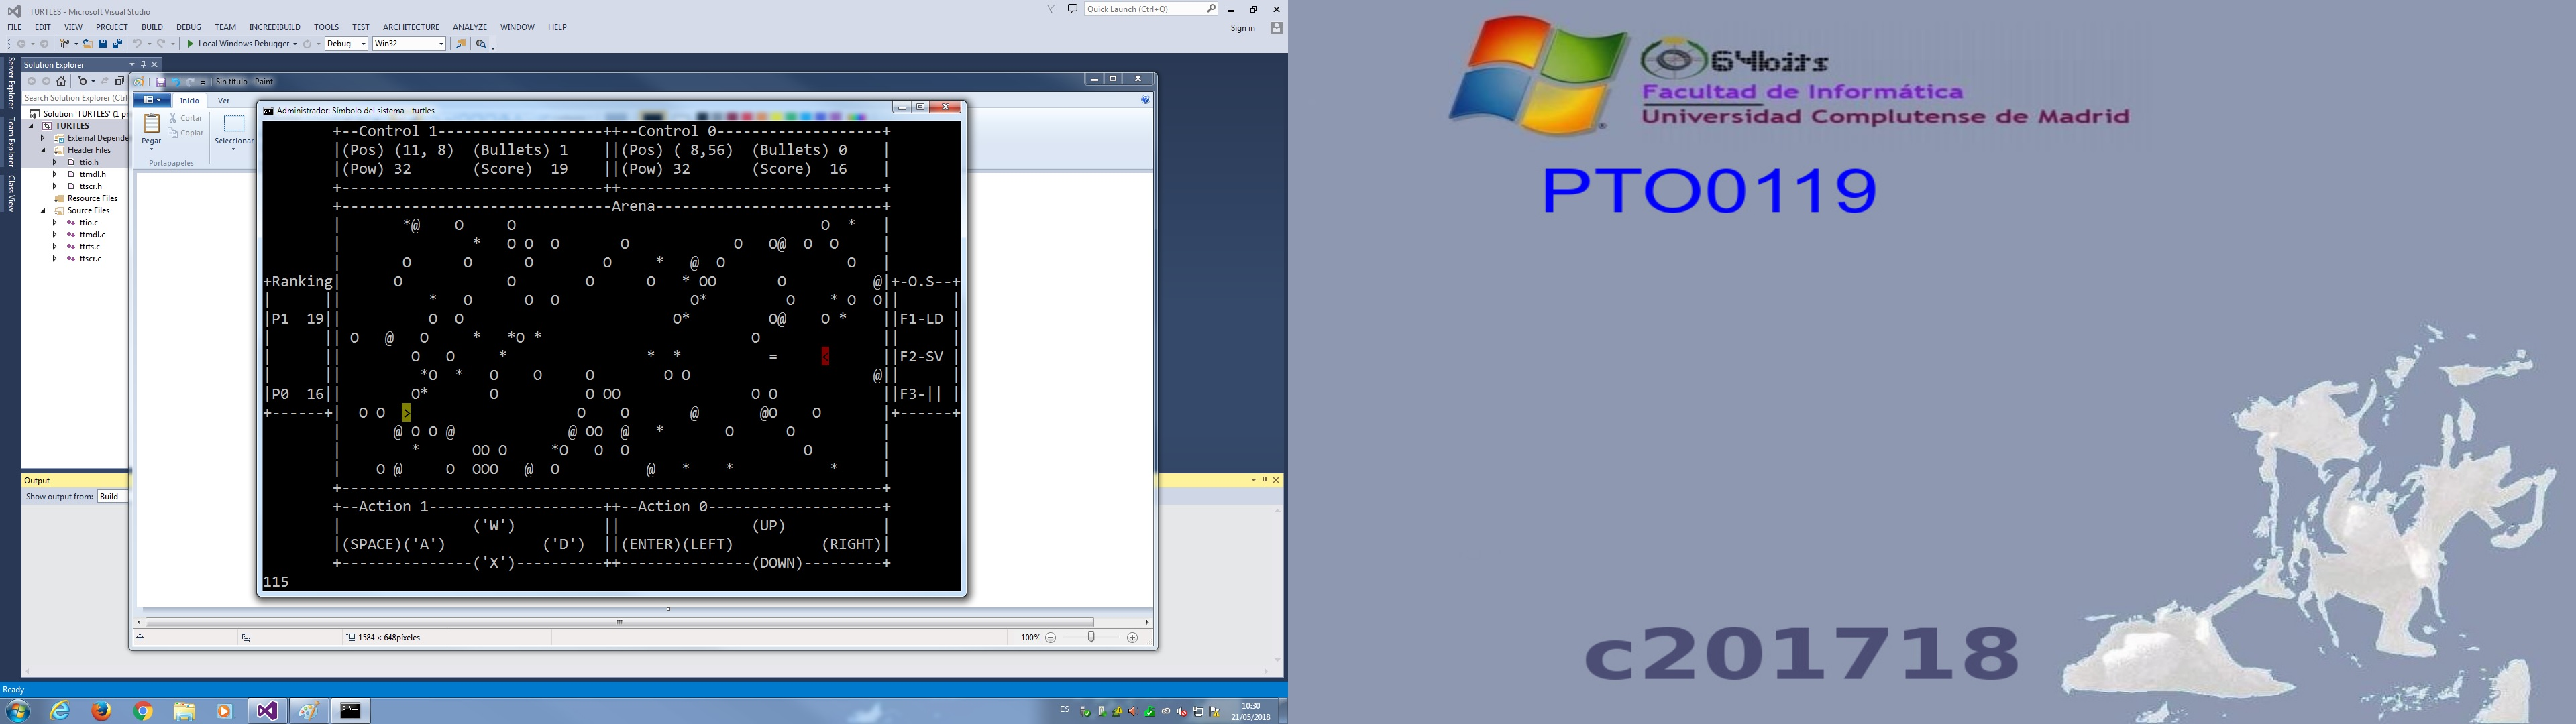
\includegraphics[scale=0.65]{res/snapshot.png}
  \end{figure}
\end{comment}
\section{Requirements and Analysis}
\label{sec:anal}


Some choices has been made to increase game's quality for playing
(\emph{playability}), with respect to table-board game.
\begin{itemize}
\item Only \emph{shooting} and \emph{moving} cards (no
  \emph{rotating}). Game control 

  \begin{itemize}
  \item \(\leftarrow, \rightarrow, \uparrow, \downarrow\) plus
    \texttt{INTRO} on right-player, or
  \item  \texttt{'A','D','W','X'} plus \texttt{SPACE} on
    left-player.
  \end{itemize}

\item Cards are not \emph{present} as in table-board
  version. Therefore \emph{they are simulated}.  Check their status at
  every player's \texttt{Control Section} area.  As you run faster,
  your \emph{power} decreases and must stop to restore. The same
  applies to bullets (\texttt{'='}). (Idea as \DOM)
\item Neither Glaces (\texttt{'*'}) nor Stones (\texttt{'O'})can be passed-through. 
\item Stones (\texttt{'O'})can be pushed.
\item Score increases when you get a jewel (\texttt{'@'}).
\item Both Glaces (\texttt{'*'}) and Turtles (\texttt{'>'})can be
  shoot. Game is over when your turtle (or other's) is shoot.
\end{itemize}

\section{Design}
\label{sec:desgn}

Four modules standing:

\begin{itemize}
\item \texttt{ttrts} ``Turtle runtime system''. Intended to process
  user's actions and dispatch them for service  routines (Event loop )
\item \texttt{ttmdl} ``Turtle model system'' .  The model of the
  application. Only \emph{two state variables} needed.

\begin{verbatim}
TURTLE *turtle[MAX_PLAYERS];
BULLET *bullet[MAX_PLAYERS];
\end{verbatim}
\item \texttt{ttscr}  ``Turtle screen''. The view of the
  application. Controlled by \ncurses library under
\begin{verbatim}
WINDOW *mainwin;
\end{verbatim}
  
\item \texttt{ttio} ``Turtle IO services''. Initially interface with
  IO routines for saving, restoring game, etc... Then implementing
  Time Event emulation, both with signal handlers for \texttt{Linux}
  and \texttt{Microsoft}.
\end{itemize}


\section{Coding}
\label{sec:code}
Easier Code... Almost every routine is \(O(1)\)
\section{Conclusions}
\label{sec:conc}

Bla,bla...
\newpage

\appendix{\textbf{APPENDIX. curses library}}
\label{sec:curses}

Refer to ...




\begin{thebibliography}{}
\bibitem{rockkind} Marck J. Rochkind:
  \emph{Advanced C Programming for Displays},
  Prentice Hall, Englewood Cliffs, N.J 07632
\end{thebibliography}
\end{document}

%%% Local Variables:
%%% mode: latex
%%% TeX-master: t
%%% End:
